\documentclass[11pt,]{article}
\usepackage[left=1in,top=1in,right=1in,bottom=1in]{geometry}
\newcommand*{\authorfont}{\fontfamily{phv}\selectfont}
\usepackage[]{mathpazo}


  \usepackage[T1]{fontenc}
  \usepackage[utf8]{inputenc}



\usepackage{abstract}
\renewcommand{\abstractname}{}    % clear the title
\renewcommand{\absnamepos}{empty} % originally center

\renewenvironment{abstract}
 {{%
    \setlength{\leftmargin}{0mm}
    \setlength{\rightmargin}{\leftmargin}%
  }%
  \relax}
 {\endlist}

\makeatletter
\def\@maketitle{%
  \newpage
%  \null
%  \vskip 2em%
%  \begin{center}%
  \let \footnote \thanks
    {\fontsize{18}{20}\selectfont\raggedright  \setlength{\parindent}{0pt} \@title \par}%
}
%\fi
\makeatother




\setcounter{secnumdepth}{3}


\usepackage{graphicx,grffile}
\makeatletter
\def\maxwidth{\ifdim\Gin@nat@width>\linewidth\linewidth\else\Gin@nat@width\fi}
\def\maxheight{\ifdim\Gin@nat@height>\textheight\textheight\else\Gin@nat@height\fi}
\makeatother
% Scale images if necessary, so that they will not overflow the page
% margins by default, and it is still possible to overwrite the defaults
% using explicit options in \includegraphics[width, height, ...]{}
\setkeys{Gin}{width=\maxwidth,height=\maxheight,keepaspectratio}

\title{Mi playa\\
Subtítulo\\
Subtítulo  }



\author{\Large Ana Hilda Valera Arias\vspace{0.05in} \newline\normalsize\emph{Estudiante, Universidad Autónoma de Santo Domingo (UASD)}  }


\date{}

\usepackage{titlesec}

\titleformat*{\section}{\normalsize\bfseries}
\titleformat*{\subsection}{\normalsize\itshape}
\titleformat*{\subsubsection}{\normalsize\itshape}
\titleformat*{\paragraph}{\normalsize\itshape}
\titleformat*{\subparagraph}{\normalsize\itshape}

\titlespacing{\section}
{0pt}{36pt}{0pt}
\titlespacing{\subsection}
{0pt}{36pt}{0pt}
\titlespacing{\subsubsection}
{0pt}{36pt}{0pt}





\newtheorem{hypothesis}{Hypothesis}
\usepackage{setspace}

\makeatletter
\@ifpackageloaded{hyperref}{}{%
\ifxetex
  \PassOptionsToPackage{hyphens}{url}\usepackage[setpagesize=false, % page size defined by xetex
              unicode=false, % unicode breaks when used with xetex
              xetex]{hyperref}
\else
  \PassOptionsToPackage{hyphens}{url}\usepackage[unicode=true]{hyperref}
\fi
}

\@ifpackageloaded{color}{
    \PassOptionsToPackage{usenames,dvipsnames}{color}
}{%
    \usepackage[usenames,dvipsnames]{color}
}
\makeatother
\hypersetup{breaklinks=true,
            bookmarks=true,
            pdfauthor={Ana Hilda Valera Arias (Estudiante, Universidad Autónoma de Santo Domingo (UASD))},
             pdfkeywords = {dinámica costera, \emph{beachrock}, manglar,erosión, playa},  
            pdftitle={Mi playa\\
Subtítulo\\
Subtítulo},
            colorlinks=true,
            citecolor=blue,
            urlcolor=blue,
            linkcolor=magenta,
            pdfborder={0 0 0}}
\urlstyle{same}  % don't use monospace font for urls

% set default figure placement to htbp
\makeatletter
\def\fps@figure{htbp}
\makeatother

\usepackage{pdflscape} \newcommand{\blandscape}{\begin{landscape}}
\newcommand{\elandscape}{\end{landscape}}


% add tightlist ----------
\providecommand{\tightlist}{%
\setlength{\itemsep}{0pt}\setlength{\parskip}{0pt}}

\begin{document}
	
% \pagenumbering{arabic}% resets `page` counter to 1 
%
% \maketitle

{% \usefont{T1}{pnc}{m}{n}
\setlength{\parindent}{0pt}
\thispagestyle{plain}
{\fontsize{18}{20}\selectfont\raggedright 
\maketitle  % title \par  

}

{
   \vskip 13.5pt\relax \normalsize\fontsize{11}{12} 
\textbf{\authorfont Ana Hilda Valera Arias} \hskip 15pt \emph{\small Estudiante, Universidad Autónoma de Santo Domingo (UASD)}   

}

}








\begin{abstract}

    \hbox{\vrule height .2pt width 39.14pc}

    \vskip 8.5pt % \small 

\noindent Mi resumen


\vskip 8.5pt \noindent \emph{Keywords}: dinámica costera, \emph{beachrock}, manglar,erosión, playa \par

    \hbox{\vrule height .2pt width 39.14pc}



\end{abstract}


\vskip 6.5pt


\noindent  \section{Introducción}\label{introducciuxf3n}

El mar constituye un elemento fundamental del conjunto de componentes de
la superficie terrestre, capaz de generar cambios en las líneas de
costas, sean estas en una isla o continente de acuerdo con (Kokot,
Codignotto, \& Elissondo, 2004). Para Suárez de Vivero (1999), el
término costa puede aludir a la franja de tierra que bordea el mar o a
la zona de contacto entre el medio marino y el medio terrestre. Teniendo
en cuenta que la línea de costa puede variar en un instante, o con el
paso de los años, ya sea por la dinámica litoral o por causa de
fenomenos naturales, que pueden traer como posible concecuencia la
erosión o regresión de la costa (J. Codignotto, 1997; Kokot, 2004).

Para Kokot (2004), la erosión costera es el resultado de un exceso de
remoción de sedimentos respecto del aporte suministrado a un área
determinada en un periodo específico. La misma abarca la emersión y
sumersión de sedimentos en las orillas del mar o la playa, lo que
mantiene en constante movimiento el límite exacto de la costa. Varios
autores se han dedicado al análisis de línea de costa, usando como
fuentes imágenes satélitales o fotografías áereas históricas. También se
realizan observaciones y mediciones por un periodo de tiempo determinado
que puedan dar respuesta a las causas de dicho cambio ({\textbf{???}};
Esquer, Carreon, \& others, 2018; Hernández Santana, Ortiz Pérez, Méndez
Linares, \& Gama Campillo, 2008).

La costa como unidad geomorfológica se mantiene en constante estado de
evolución. La importancia de conocer hacia dónde se desplaza más y qué
forma ésta va adquiriendo, permite diferenciar el tipo de costa que, de
acuerdo con J. Codignotto (1997), puede clasificarse como: costa en
progradación, costa estacionaria y costa en retrogradación. Del mismo
modo, el autor hace énfasis en la importancia de comprender los factores
que iniciden en este proceso y las causas que lo producen. Además de
incluir posibles formaciones geoquimicas que se pueden producir en la
zona producto de estos cambios, como es el caso de la roca de playa.

De acuerdo con Aliotta, Spagnuolo, \& Farinati (2009), las rocas o
\emph{beachrock} son formaciones sedimentológicas comunes que evidencian
un proceso erosivo del litoral, los cuales se dieron lugar en un
ambiente geoquímico que enmarcó un periodo de evolución continua que
pudo abarcar varias etapas del tiempo geológico. Es posible que durante
ese proceso la arena de la playa compactara por medio de cemento
carbonático y al pasar varias épocas posiblemete afloraron. En la isla
de Santo Domingo las formaciones arrecifales o rocas de playas datan del
Neógeno y el periodo cuaternario. Ejemplo de ella según Diaz de Neira
(2007--2010), la Fm. Isabela del pleistoceno; formación carbonatada
arrecifal, rica en corales de tallas variables. Aflora bajo la forma de
diferentes relieves, formando arrecifes en escalera descendiendo hacia
el mar.

El litoral costero de la parte sur del país se caracteriza por pequeños
acantilados, playas de origen aluvial y dunas extensas (Abreu, 1999).
Además, mareas con oleajes extremos típico del mar caribe. No obstante,
la ecología actúa como componente categórico en el microclima de una
zona, resultado de la diversidad que ésta puede aportar. Por tal motivo,
el interés de conocer el tipo de vegetación. Razón de que estos, sobre
la arena son imprescindible para la conservación de los sedimentos, los
cuales pueden desvanecerse a concecuencia de la erosión del viento y la
lluvia (D'Croz, 1985).

De acuerdo con Cámara Artigas (1997), los litorales de la isla, se
caracterizan por tener plantas propias de la familia Polygonaceae o
Rhizophoraceae como la cocoloba\_uvífera (uva de playa) (ver figura
\ref{cocoloba}) y el mangle rojo (ver figura \ref{manglerojo}). De igual
modo la vegetación cercanas a aguas dulce o salada suele llamarse
bosques de manglares, estos suelen encontrarse en algunas dunas costeras
de la parte sur del país, principalmente en las riveras y desembocaduras
de cuencas lacustre. Conforme Polanía \& Nat (1998), estos tipos de
bosques son asociaciones vegetales que prosperan en las costas
tropicales y subtropicales del mundo. Pero en la isla de Santo Domingo
existe una tipología diferente en dichos espacios costeros.

La playa de Najayo se encuentra ubicada en la sección del mismo nombre,
perteneciente al municipio San Gregorio de Nigua, provincia San
Cristóbal, al Sur de la República Dominicana. Fisiográficamente, se
ubica en la llanura costera del Caribe, en las coordenadas aproximadas
18º17'40" latitud Norte y 70º06'02" longitud Oeste. De acuerdo al mapa
geológico de la isla de Santo Domingo (Abad de los Santos, 2007--2010),
se estima que la formación del relieve costero de Najayo data de la era
Cenozoica periodo Cuaternario entre las época Eoceno-Mioceno, el mismo
está compuesto por arena y gravas bioclásticas formando el cordón
litoral, además de conglomerado, gravas, arenas de fondo de valle,
calizas arrecifales, calciruditas y calcarenitas (ver figura
\ref{mapageo50k}).

\begin{figure}
\centering
\includegraphics{Cocoloba_uvifera.jpg}
\caption{Vegetación dunas de playa\label{cocoloba}}
\end{figure}

\begin{figure}
\centering
\includegraphics{mangle_rojo.png}
\caption{Vegetación riveras de playa-río\label{manglerojo}}
\end{figure}

\begin{figure}
\centering
\includegraphics{mapa_bahia_najayo.png}
\caption{Mapa geológico escala 1:50,000 (hoja Nizao)\label{mapageo50k}}
\end{figure}

\ldots

\section{Metodología}\label{metodologuxeda}

Para el análisis de cambio en la línea costera de la playa Carlos Pinto,
ubicada en el paraje del mismo nombre, zona Oeste de la sección Playa
Najayo provincia San Cristóbal. Se utilizó como referencia de estudio
imágenes satélitales de Landsat 5, 7 y 8, de los años
(2013,2014,2015,2016,2017,2018 y 2019). Las cuales fueron delimitadas
empleando el algoritmo de CoastSates que de acuerdo con Elsevier (n.d.)
es un conjunto de herramientas que posee un software de código abierto
escrito en Python que permite al usuario obtener series de tiempo,
pueden ser estos de 30 o más años, en cuanto a la posición de una costa
sin importar que sea de tipo arenosa y a nivel mundial. Dicho software
toma como base de datos imágenes satélitales disponibles al público.
También se colectaron arenas y gravas en varios punto de la costa, donde
se llenó un formulario y se tomó las coordenadas geográficas de cada
punto por medio de la aplicación ODK Collection descargada en un
dispositivo móvil. Tales puntos fueron identificado por áreas con
respecto al mar o la playa (Berma y Dunas de Playa). Los clastos
colectados fueron medidos en dos ejes (ancho y largo), de tal modo los
resultados obtenidos fueron expresados en milímetros (mm). De igual
manera se realizaron fotografias mediante la cámara de un teléfono móvil
a la vegetación y a la roca cercana a la zona de estudio.

\ldots

\section{Resultados}\label{resultados}

Los datos generados mediante el algoritmo mensionado con anterioridad,
para la recreación de línea costera y las muestras de sedimentos
colectadas en varios puntos de muestreo, así como la vegetación y las
rocas expuestas en toda la zona costera. Permite identificar y analizar
el tipo de costa que en la actualidad la playa de Carlos Pinto presenta
y por consiguiente, el modelo de material sedimentario predominante.
Además de determinar el prototipo de vegetación más abundante y como
está distribuida la roca de playa (\emph{beachrock}) en el lugar.

Cambio línea de costa

Por medio de la imágenes satélitales de landsat 5,7 y 8, entre los años
2013 hasta el 2019, se hicieron 25 transectos en toda la costa de la
playa de Najayo (ver figura \ref{transect_linea}), con la finalidad de
efectuar un análisis entre todos. El objetivo, determinar si la costa
esta padeciendo un proceso de retrogradación, progradación o es
estacionaria con el pasar del tiempo, a parte de observar cuál es la
zona que más cambio ha experimentado en este proceso (ver figura
\ref{cambio_transecto}).

La figura 4 muestra los 25 transectos realizados sobre las diferentes
líneas, las mismas hacen alusión al límite entre el espacio terrestre y
el espacio acuático en un determinado periodo de año. En tanto que la
figura 5 muestra los diferentes transectos haciendo énfasis en el tipo
de forma que a adquirido el litoral en un tiempo específico (cada 3
meses).

De acuerdo a la figua 5 se puede observar que en el año 2013, el primer
y segundo trimestre el mar retrogradó poco menos de 20 metros, con
excepción en los transectos número 1,2,7,8,10,15,23 los cuales no
muestran cambio significativos en el desplazamiento de las líneas y el
transecto número 14 donde el mar obtuvo una ligera agradación. En cuanto
el tercer y cuarto trimestre muestra una notable agradación de parte de
la tierra firme hacia el mar, como es el caso en los transectos
1,6,14,15,16,17,18,19 y 25, mientras que los demás no obtuvieron
alteración importante.

Mientras que en el año 2014, en el primer trimestre la tierra agradó
poco menos de 20 m en los transectos 1,6,14,15,19 y 25 en comparación
con los demás que su variación fue mínimo o nulo. En el segundo
trimestre el mar retrogadó igual o poco menos de 20 m en los transectos
17,18,20,22,24 y 25, en tanto que en los restante la variabilidad fue
exiguo. En cuanto, en el tercer trimestre la tierra prosperó hacia el
mar, de acuerdo a los transectos 1,14,16,18,19 y 25 poco o igual a 20
m., entretanto en los otros transectos la transformación fue
insignificante. Mientras tanto en el cuarto trimestre la tierra produjo
un avance hacia el mar en los transectos 1,14,15,18,19 y 25 de 20 m o
menos, en relación con los damás que sus alteraciones fueron pequeñas o
inexistentes.

Para el año 2015, el primer trimestre presenta una marcada agradación de
parte de la tierra en los transectos 1,16,18,19 y 25 a una distancia
igual o menor de 20 m., mientras que en los demás punto la vicisitud es
muy baja o nula. En el segundo trimestre la tierra avanzó hacia el mar
en los transectos 1,5,13,17,18 y 25 poco menos de 20 M, entre tanto, los
demás transectos presentan variaciones insignificante o ninguna. En
cuanto que, en el tercer trimestre el mar obtuvo una retrogradación
relevante, poco menos de 20 m en los transectos 16,17,19,24 y 25, en
tanto que en los otros puntos el cambio fue mínimo. En el cuarto
trimestre la alteración presentada por los transectos en la línea de
costa se encuentran en los punto 1,17 y 25 los cuales tienen una
distancia poco menos de 20 m, mientras que los transectos restantes
poseen muy bajos o ninguna variabilidad.

En el primer trimestre del año 2016, sólo los transectos 1 y 25 muestra
una ligera agradación de la tierra hacia el mar de igual o menos a los
20 m, en tanto que los otros no muestran cambios importantes. Para el
segundo trimestre los transectos muestran una variedad muy expresiva en
los números 3,4,5,16,17,19,20,21,22,24 y 25 con un espacio de poco o
igual a 20 m., en cuanto el avance del mar hacia tierra firme, mientras
que los demás transectos no presentan cambios relevantes. De acuerdo al
tercer trimestre los cambios fueron muy mínimo o nulo. Por ejemplo, los
transectos 1,5,13 y 20 son los que presenta una pequeña variabilidad de
costa. Donde la tierra firme prospera al mar a una distancia menor a los
20 m. En tanto que el cuarto trimestre los transectos 1,13,15,17 y 25
muestran una transición de parte de la tierra hacia el mar de poco menos
de 20 m, en comparación con los demás puntos, que no presentan cambios
sustanciales.

En el año 2017, el primer trimestre presenta un pequeño cambio en los
transectos, donde se observa que la tierra progresa hacia al mar a una
distancia de 20 m o menos en los transectos 1,13,14,15 y 16, mientras
que en los demas transectos la diferencia es nula. En el sugundo
trimestre los distinto lugares en la costa presentan ligera transición
de parte del mar hacia la tierra en los puntos 19,20 y 24, en relación a
los otros que no presentan cambios significativos. Mientras tanto el
tercer trimestre no presenta variación considerable entre los diferentes
transectos. En cuanto al cuarto trimestre los punto 15,17 y 25 alumbran
una variabilidad mínima en la agradación realizada por la tierra hacia
al mar, por consiguiente los demás espacio restantes no presentan
variación en la costa.

El año 2018 el primer trimestre presenta transectos con alteración
valiosa en la costa, los transectos 1 y 25 muestran una agradación de la
tierra de poco menos de 20 m con relación al mar, mientras que el
transecto 16 presenta una retrogradación de parte del mar hacia la
tierra de poco menos de 20 m, en tanto los demás punto no muestran
cambio importante. El segundo trimestre presenta transformación en la
costa de acuerdo a los transectos, donde el mar presenta una
retrogradación en los puntos 15,16,17,18,19,20,24 y 25 con distancia
igual o menor a 20 m, mientras tanto en los demás punto la variación es
mínima o inexistente. En el tercer trimestre solo los transectos 15,19 y
20 muestran ligeras transiciones menores a 20 m., en tanto los otros no
presentan alteraciones valiosas. De igual forma el cuarto trimestre
prenta cambio en el transecto 1, donde la tierra avanza hacia el mar
poco menos de 20 m y el punto 24 donde el mar prospera hacia tierra
firme poco menos de 20 m., entretanto los demás no presentan algún
traslado en la línea de costa.

Por último el año 2019, donde el primer trimestre muestran variedad en
los transectos sobre la línea de costa en los números 1,17 y 25 en los
cuales la tierra avanza hacia el mar poco menos de 20 m, mientras que en
los punto 16,18,19 y 24 existe una retrogradación de parte del mar hacia
la tierra poco menos de 20 m., en tanto que los demás no muestran cambio
considerables. El segundo trimestre muestra visicitudes notables entres
los transectos con relación a la línea de costa. Los puntos
4,5,16,17,19,21,24 y 25 presentan un avance del mar hacia la tierra de
menor o igual a 20 m., por otra parte el transecto 1 muestra una
agradación de la tierra hacia el mar poco menos de 20 m, mientras tanto
los demás no muestran variaciones significativas. En el tercer y cuarto
trimestre no existe una alteración considerable en los transectos sobre
las líneas costera.

Roca de playa (\emph{beachrock})

La playa de Najayo presenta un pequeño acantilado en medio de la costa,
a parte de exhibir afloramiento de rocas en algunos lugares, sean estos
a orrillas o dentro del mar (ver figura \ref{beachrock}), siendo el
espacio visiblemente más afectado la parte central de la costa.

Vegetación

La vegetación en la duna de la playa de Carlos Pinto predomina la
cocoloba\_uvífera y la ipomoea\_pescabrea. En tanto que, en la
desembocadura del arroyo agua dulce (ver figura \ref{arroyo_aguadulce})
existe un bosque tipo manglar en el cual se destaca el mangle blanco,
mientras que el acantilado muestra una flora muy heterogéna, donde
prevalece el noni, almácigo, eugenia, mara entre otros.

\begin{figure}
\centering
\includegraphics{transect_linea_R.png}
\caption{Transectos sobre las líneas costera de
playa\_Najayo\label{transect_linea}}
\end{figure}

\begin{figure}
\centering
\includegraphics{cambio_playa_Najayo.png}
\caption{Transectos sobre las líneas costera de
playa\_Najayo\label{cambio_transecto}}
\end{figure}

\begin{figure}
\centering
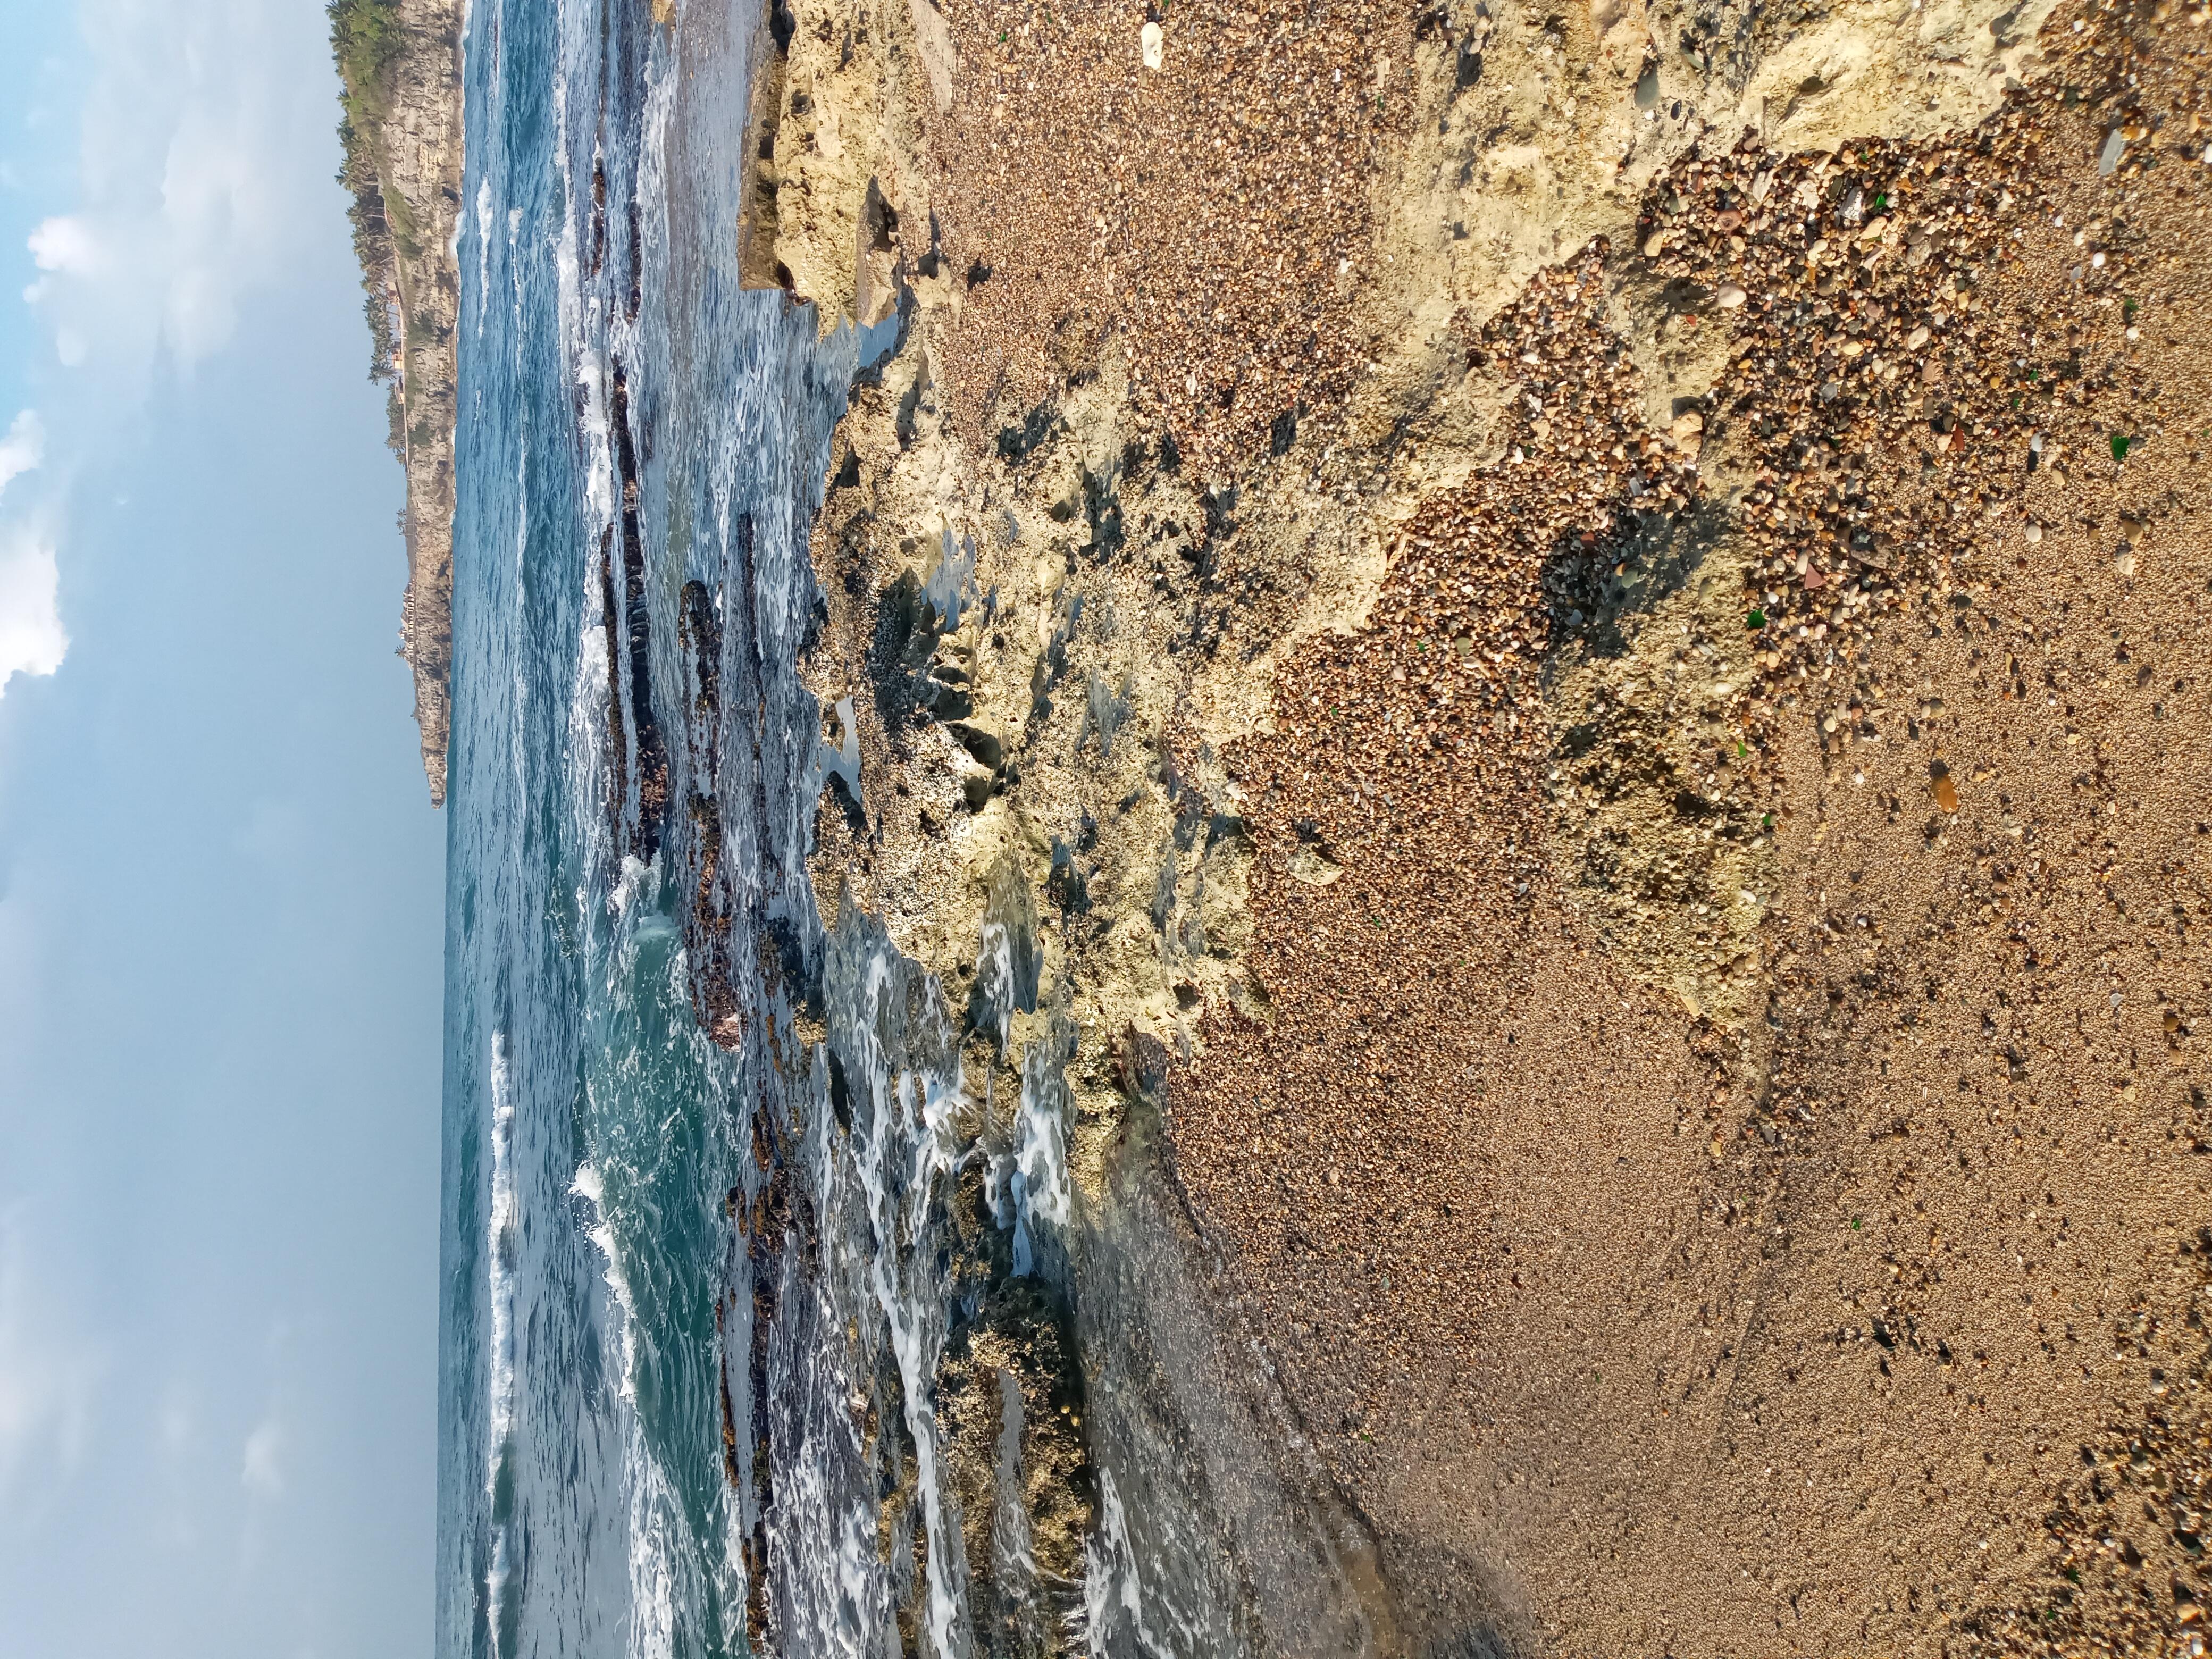
\includegraphics{Beachrock.jpg}
\caption{Afloramiento de rocas playa\_Najayo\label{beachrock}}
\end{figure}

\begin{figure}
\centering
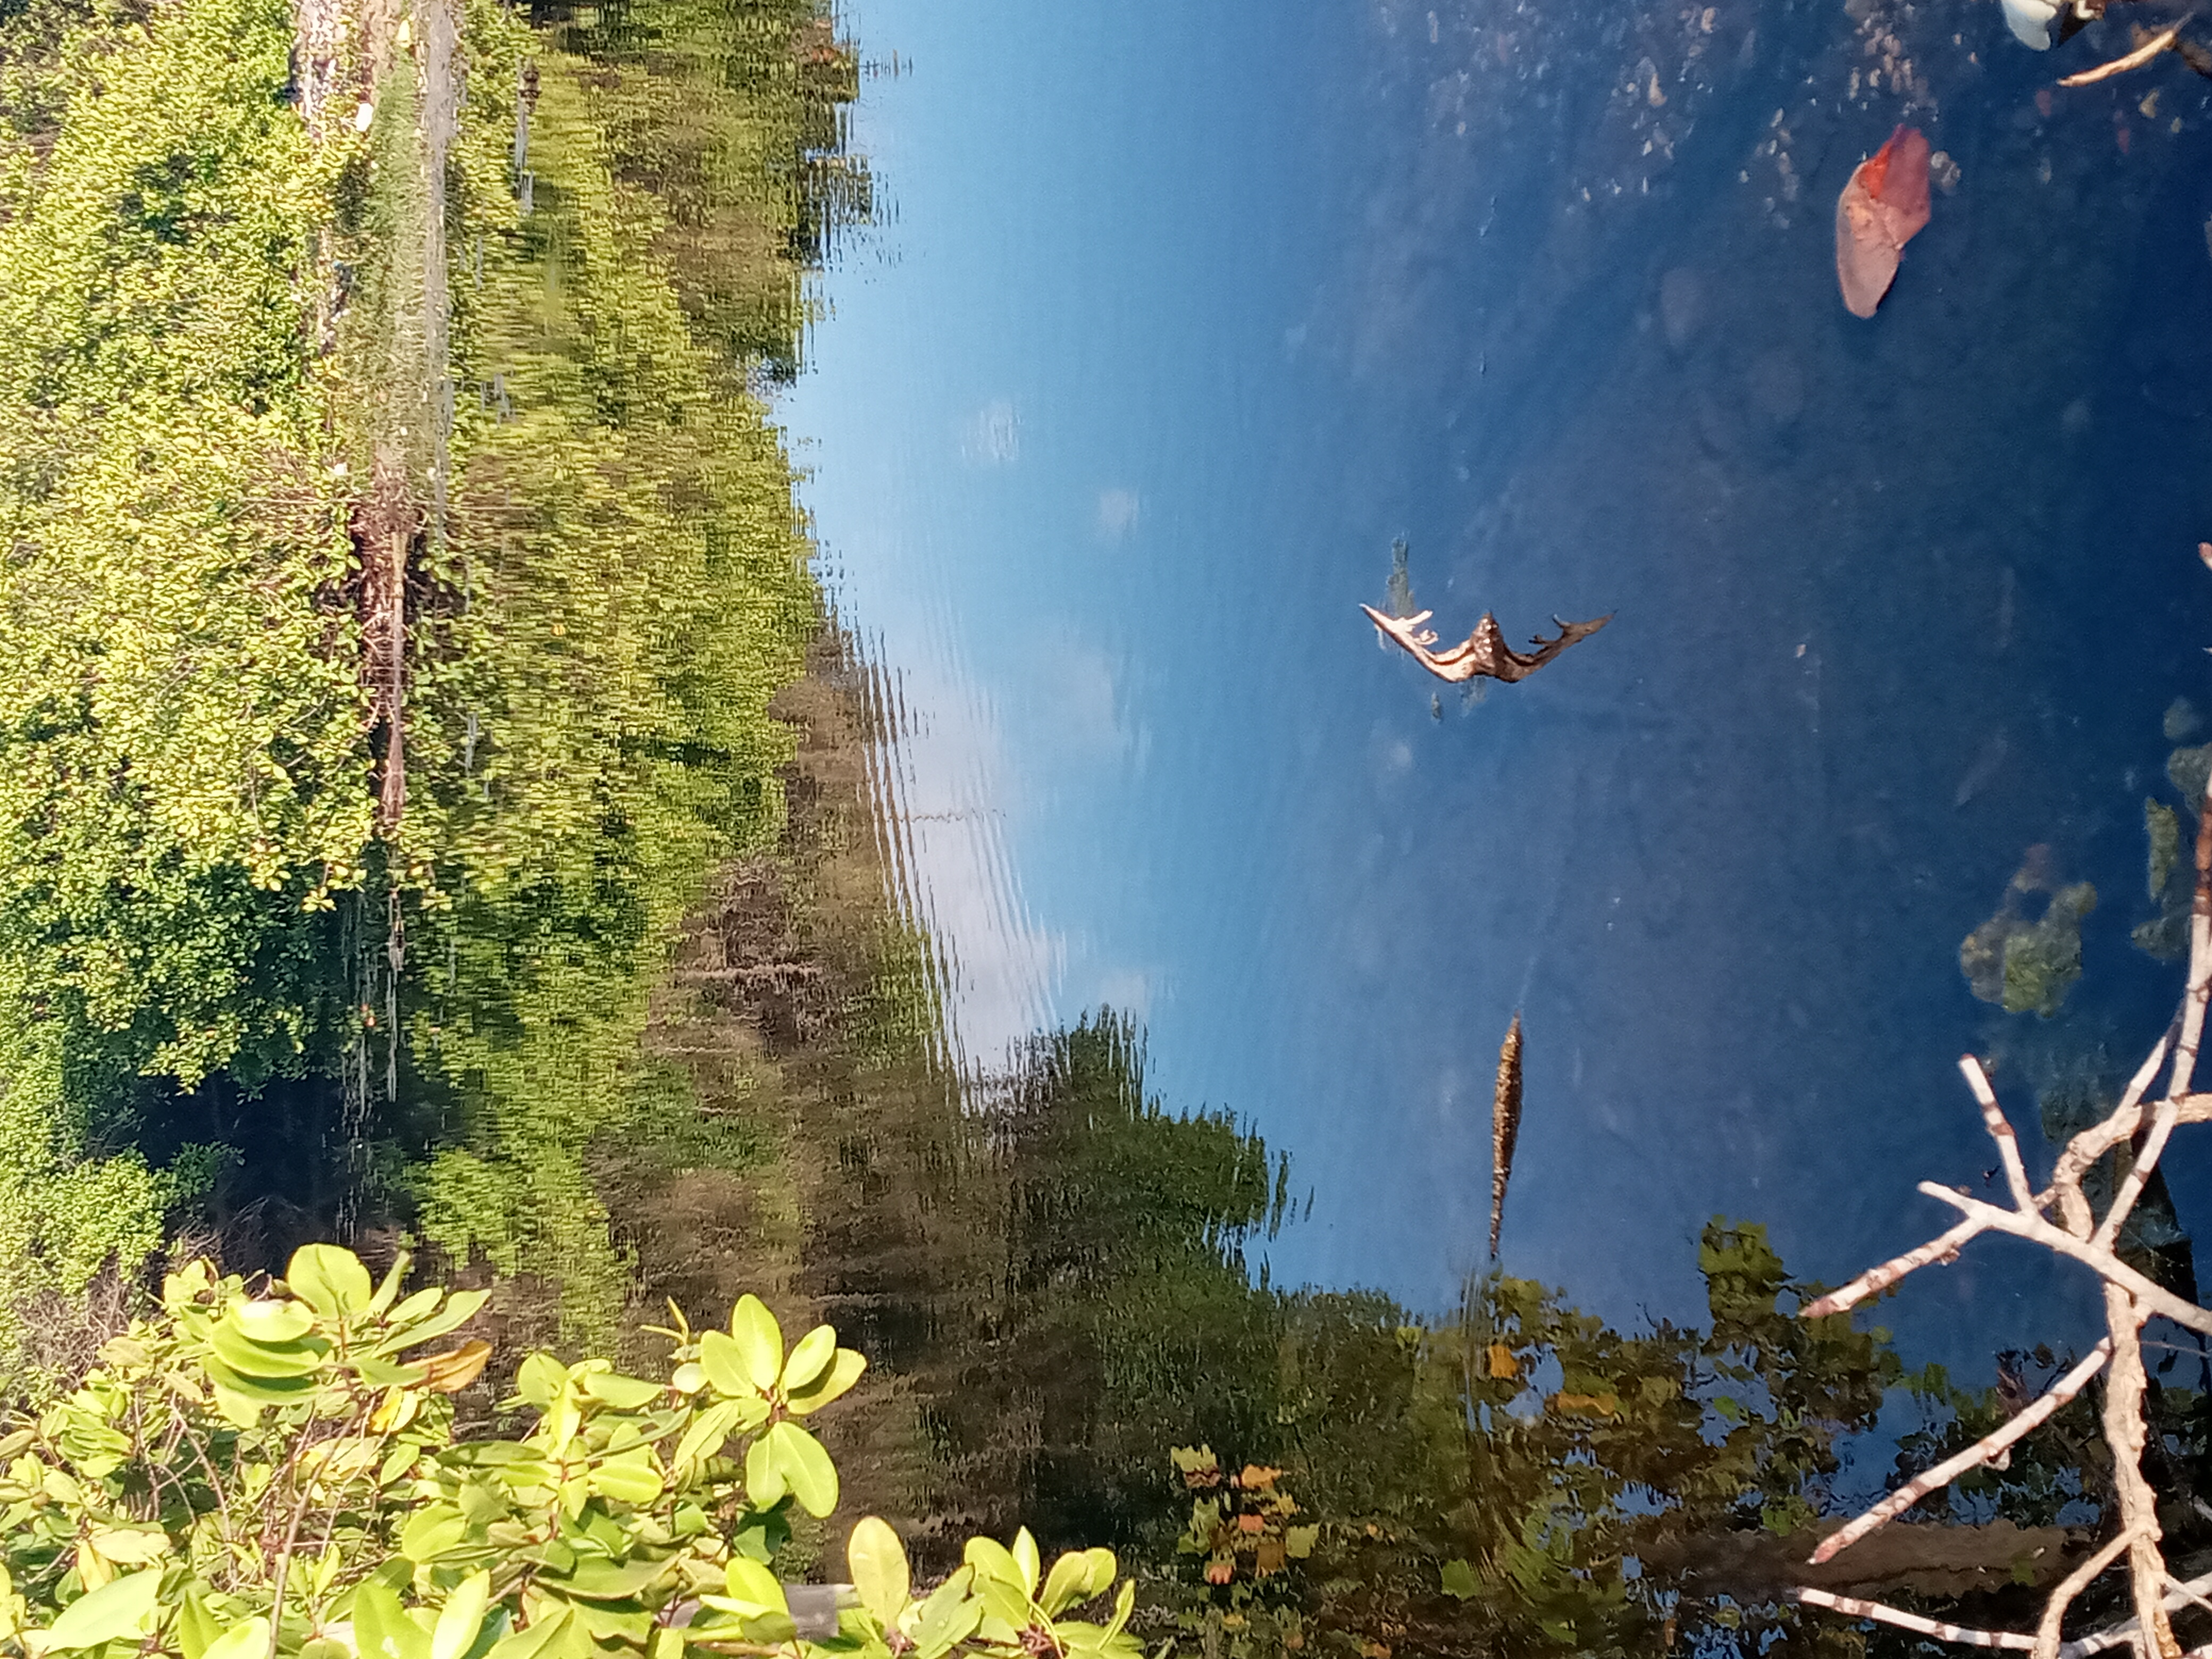
\includegraphics{Arroyo_Aguadulce.jpg}
\caption{Desembocadura arroyo Agua Dulce
Playa\_Carlos\_Pinto\label{arroyo_aguadulce}}
\end{figure}

\ldots

\section{Discusión}\label{discusiuxf3n}

\section{Agradecimientos}\label{agradecimientos}

\section{Información de soporte}\label{informaciuxf3n-de-soporte}

\ldots

\section{\texorpdfstring{\emph{Script}
reproducible}{Script reproducible}}\label{script-reproducible}

\ldots

\section*{Referencias}\label{referencias}
\addcontentsline{toc}{section}{Referencias}

\hypertarget{refs}{}
\hypertarget{ref-abad2007mapageonizao}{}
Abad de los Santos, M. (. (2007--2010). \emph{Mapa Geológico de la
República Dominicana a escala 1:50.000 de la hoja n 6170-I (Nizao) y
Memoria correspondiente}. Santo Domingo: Proyecto 1B de Cartografía
Geotemática de la República Dominicana. Programa SYSMIN. Servicio
Geológico Nacional.

\hypertarget{ref-abreu1999impacto}{}
Abreu, L. (1999). Impacto del turismo en el litoral de dominicana.
\emph{Revista Geográfica}, 167--182.

\hypertarget{ref-aliotta2009origen}{}
Aliotta, S., Spagnuolo, J. O., \& Farinati, E. A. (2009). Origen de una
roca de playa en la región costera de bahía blanca, argentina.
\emph{Pesquisas Em Geociências}, \emph{36}(1), 107--116.

\hypertarget{ref-camara1997republica}{}
Cámara Artigas, R. (1997). \emph{República dominicana: Dinámica del
medio físico en la región caribe (geografía física, sabanas y litoral)
aportación al conocimiento de la tropicalidad insular}.

\hypertarget{ref-codignotto1997geomorfologia}{}
Codignotto, J. (1997). \emph{Geomorfología y dinámica costera}.

\hypertarget{ref-maparecursosminerales}{}
Diaz de Neira, A. (2007--2010). \emph{Mapa de recursos minerales de la
Repú Dominicana, escala 1:100,000}. Santo Domingo: Proyecto 1B de
Cartografía Geotemática de la República Dominicana. Programa SYSMIN.
Servicio Geológico Nacional.

\hypertarget{ref-d1985manglares}{}
D'Croz, L. (1985). Manglares: Su importancia para la zona costera
tropical. \emph{Agonia de La Naturaleza}, 167--180.

\hypertarget{ref-vos2019coastsat}{}
Elsevier (Ed.). (n.d.). CoastSat: Un kit de herramientas python
habilitado para google earth engine para extraer costas de imágenes
satelitales disponibles públicamente. \emph{Environmental Modeling ~\&
Software}.

\hypertarget{ref-esquer2018modificacion}{}
Esquer, M. Z., Carreon, T. E., \& others. (2018). MODIFICACION de linea
de costa. \emph{Revista de Investigación Académica Sin Frontera:
División de Ciencias Económicas Y Sociales}, (16).

\hypertarget{ref-hernandez2008morfodinamica}{}
Hernández Santana, J. R., Ortiz Pérez, M. A., Méndez Linares, A. P., \&
Gama Campillo, L. (2008). Morfodinámica de la línea de costa del estado
de tabasco, méxico: Tendencias desde la segunda mitad del siglo xx hasta
el presente. \emph{Investigaciones Geográficas}, (65), 7--21.

\hypertarget{ref-kokot2004erosion}{}
Kokot, R. R. (2004). \emph{Erosión en la costa patagónica por cambio
climático}.

\hypertarget{ref-kokot2004vulnerabilidad}{}
Kokot, R. R., Codignotto, J. O., \& Elissondo, M. (2004).
\emph{Vulnerabilidad al ascenso del nivel del mar en la costa de la
provincia de río negro}.

\hypertarget{ref-polania1998manejo}{}
Polanía, J., \& Nat, R. (1998). Manejo de ecosistemas de manglar.
\emph{Memorias Del Curso Manejo de Ecosistemas de Manglar Y Arrecifes de
Coral. Bogotá}, 153--168.

\hypertarget{ref-suarez1999delimitacion}{}
Suárez de Vivero, J. L. (1999). Delimitación y definición del espacio
litoral. \emph{Jornadas Sobre El Litoral de Almería: Caracterización,
Ordenación Y Gestión de Un Espacio Geográfico Celebradas En Almería, 20
a 24 de Mayo de 1997. Pag: 13-23}.




\newpage
\singlespacing 
\end{document}
